\section{REALIS}\label{Sec:REALIS}

Wird vom Buisness bei Infineon für einen Kunden ein neues Produkt angefordert, oder entwickeln diese selber ein neues Produkt, so muss dieses erst einmal getestet werden, bevor es in Masse produziert werden kann. Mit Produkt meine ich dabei, einen fertigen Chip, der auf einem Wafer gefertigt wurde. Für diese Zuverlässigkeits-Tests wurde bei Infineon eine Software entwickelt mit dem namen \acf{REALIS}. Dieser System umfasst die komplette Planung und Dokumentation der Durchführung und Ergebnisse dieser Tests. 



\subsection{REALIS - Project Life Cycle}

Um ein neues Produkt zu testen, wird vom sogenannten \ac{QM} bei Infineon ein neues Projekt in \ac{REALIS} angelegt \todo{oder auch eQTP ?}. Dieses befüllt er mit verschiedenen (Stress)-Tests, basierend auf vorhandenen Templates, die Arbeitsschritte (Operationen), Start- und Enddaten, Parameter der Operationen einzelner Tests und weitere Informationen enthält. Dieser erste Schritt entspricht der obersten Reihe in Abbildung \ref{fig:realis-project-lifecycle} und bildet den Anfang eines REALIS Projekt-Lebenszyklus.

Im zweiten Schritt wird übergibt der \ac{QM} das Projekt durch einen internen Mechanismus, einen State-Change des Projekts, dem \ac{RPT}-Labor. RPT-Labore 


...\todo{add Facts about realis: usercount, rpt-lab count, ...}

\begin{figure}[!h]
    \centering
    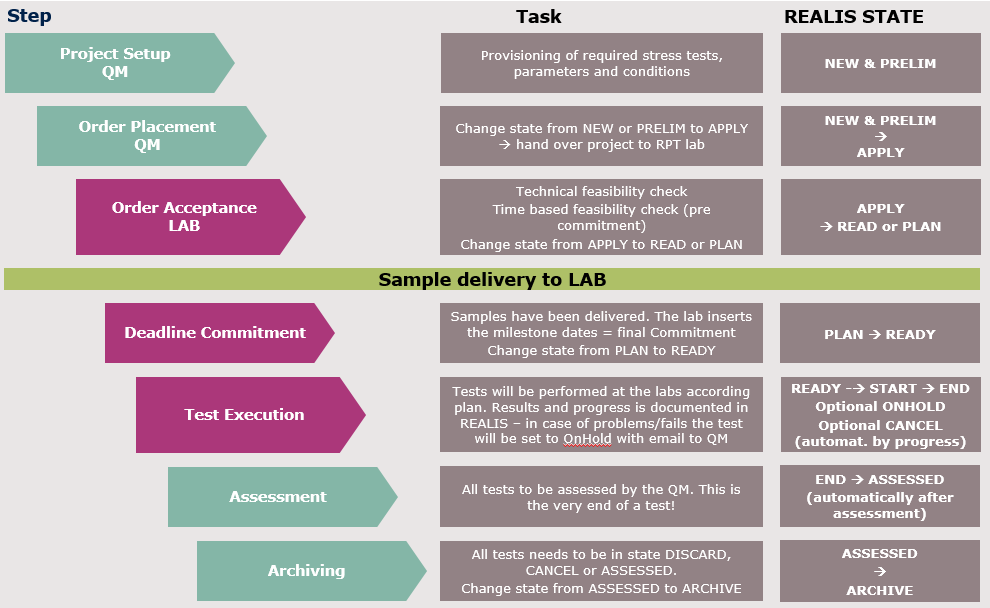
\includegraphics[width=0.9\textwidth]{bilder/realis-project-lifecycle.png}
    \caption{REALIS Project Lifecycle}
    \label{fig:realis-project-lifecycle}
\end{figure}
